% $Header: /home/vedranm/bitbucket/beamer/solutions/generic-talks/generic-ornate-15min-45min.en.tex,v 90e850259b8b 2007/0\frac{1}{2}8 20:48:30 tantau $
\documentclass{beamer}
%\documentclass[handout]{beamer}
\usefonttheme[onlymath]{serif}
% This file is a solution template for:
\usepackage{algcompatible}
\usepackage{algpseudocode}
\usepackage{multicol}
\usepackage{animate}
% - Giving a talk on some subject.
% - The talk is between 15min and 45min long.
% - Style is ornate.
% Copyright 2004 by Till Tantau <tantau@users.sourceforge.net>.
%
% In principle, this file can be redistributed and/or modified under
% the terms of the GNU Public License, version 2.
%
% However, this file is supposed to be a template to be modified
% for your own needs. For this reason, if you use this file as a
% template and not specifically distribute it as part of a another
% package/program, I grant the extra permission to freely copy and
% modify this file as you see fit and even to delete this copyright
% notice. 

\mode<presentation>
{
  \usetheme{Warsaw}
  % or ...

  \setbeamercovered{transparent}
  % or whatever (possibly just delete it)
}
\setbeamertemplate{navigation symbols}{} 

\usepackage[english]{babel}
% or whatever

\usepackage[latin1]{inputenc}
% or whatever
\useoutertheme{default}

\usepackage{times}
\usepackage[T1]{fontenc}
% Or whatever. Note that the encoding and the font should match. If T1
% does not look nice, try deleting the line with the fontenc.
\newcommand{\beforeverb}{\footnotesize}
\newcommand{\afterverb}{\normalsize}

\title[Solving Classical Equations of Motion] % (optional, use only with long paper titles)
{Lecture 12}

\subtitle
{Solving Classical Equations of Motion} % (optional)

\author[Ying-Jer Kao] % (optional, use only with lots of authors)
{Ying-Jer Kao}
% - Use the \inst{?} command only if the authors have different
%   affiliation.

\institute[National Taiwan University] % (optional, but mostly needed)
{
  Department of Physics\\
 National Taiwan University
  }
% - Use the \inst command only if there are several affiliations.
% - Keep it simple, no one is interested in your street address.

\date[Numerical Analysis and Programming] % (optional)
{\today}

\subject{Talks}
% This is only inserted into the PDF information catalog. Can be left
% out. 



% If you have a file called "university-logo-filename.xxx", where xxx
% is a graphic format that can be processed by latex or pdflatex,
% resp., then you can add a logo as follows:

% \pgfdeclareimage[height=0.5cm]{university-logo}{university-logo-filename}
% \logo{\pgfuseimage{university-logo}}



% Delete this, if you do not want the table of contents to pop up at
% the beginning of each subsection:
%\AtBeginSubsection[]
%{
%  \begin{frame}<beamer>{Outline}
%    \tableofcontents[currentsection,currentsubsection]
%  \end{frame}
%}


% If you wish to uncover everything in a step-wise fashion, uncomment
% the following command: 

%\beamerdefaultoverlayspecification{<+->}


\begin{document}

\begin{frame}
  \titlepage
\end{frame}

\begin{frame}{Outline}
  \tableofcontents
  % You might wish to add the option [pausesections]
\end{frame}


% Since this a solution template for a generic talk, very little can
% be said about how it should be structured. However, the talk length
% of between 15min and 45min and the theme suggest that you stick to
% the following rules:  

% - Exactly two or three sections (other than the summary).
% - At *most* three subsections per section.
% - Talk about 30s to 2min per frame. So there should be between about
%   15 and 30 frames, all told.
\section[Introduction]{Introduction}
\begin{frame}{Introduction}
\begin{itemize}
\item In this lecture, we will discuss the numerical solution of 
ordinary differential equations (ODEs) in classical mechanics.
\item Newton's equation of motion govern the dynamics of:
\begin{itemize}
\item {celestial bodies} in the solar system
\item ``everyday motion'': projectiles, baseballs, mechanical machines
\item  non-electronic aspects of solids, liquids and gases
\end{itemize} 
We will discuss basic numerical algorithms (discretized time axis)
\begin{itemize}
\item 1D equation, properties of different integrators
\item 2D motion, driving forces, disspation...
\end{itemize}
\end{itemize}
\end{frame}

\begin{frame}{1D motion}
\begin{itemize}
\item The simplest case is the 1D motion of a particle with mass $m$ and position $x(t)$.
\item Velocity and acceleration are defined as
\[
\dot{x}(t)=\frac{d x(t)}{d t}=v(t), \quad \ddot{x}(t)=\frac{d^2 x(t)}{d t^2}=a(t)
\]
\item Given a force $F(t)$, Newton's equation of motion is
\[ 
\ddot{x}(t)=\frac{1}{m} F(x(t), \dot{x}(t),t), 
\]
given the initial conditions $x(0)=x_0$ and $v(0)=v_0$.
\item The energy should be conserved and the algorithm should be stable (error is bound).
\end{itemize}
\end{frame}


\section{Euler's method}
\begin{frame}{Euler's method}
  \begin{itemize}
    \item The simplest numerical algorithm is Euler's method:
    \item Given the initial conditions $x(0)=x_0$ and $v(0)=v_0$, we can update the position and velocity at each time step $\Delta_t$:
    \begin{align*}
      x(t+\Delta_t) &= x(t)+v(t)\Delta_t,\\
      v(t+\Delta_t) &= v(t)+a(t)\Delta_t,
    \end{align*}
    where $a(t)=F(x(t),v(t),t)/m$.
    \item In this case, we update the position and velocity at the same time step.
    \item The algorithm is first-order accurate. The Euler algorithm is not very good in practice and  should not be used in any serious work.
  \end{itemize}
\end{frame}
\begin{frame}{Simple Harmonic Oscillator}
\centerline{\includegraphics[width=0.8\textwidth]{./eulercmp.png}}
\begin{itemize}
  \item Amplitude increases with time. Unbounded energy error.
  \item We need algorithms with bounded energy error for periodic motion.
\end{itemize}
\end{frame}

\section{Leapfrog Method}
\begin{frame}{Leapfrog Method}
  \begin{itemize}
    \item The second-order form of $x$,
    $$
    x_{n+1}=x_n+\Delta_t v_n+\frac{\Delta_t^2}{2} a_n+O\left(\Delta_t^3\right)
    $$
\item The first-order form of ${v}$ :
    $$
    v_{n+1}=v_n+\Delta_t a_n+O\left(\Delta_t^2\right)
    $$
\item
    Re-write $x$ formula as
    $$
    x_{n+1}=x_n+\Delta_t\left(v_n+\frac{\Delta_t}{2}  a_n\right)+O\left(\Delta_t^3\right)
    $$
    where we can identify "half-step" velocity 
    \[
    v_{n+\frac{1}{2}} =v_n+\frac{\Delta_t}{2} a_n+O\left(\Delta_t^2\right),\quad
    x_{n+1} =x_n+\Delta_t v_{n+\frac{1}{2}}+O\left(\Delta_t^3\right)
  \]

  \end{itemize}
\end{frame}



\begin{frame}{Leapfrog Method}
  \begin{itemize}
  
  \item We will only have $v$ on the half-step, use $v_{n-\frac{1}{2}}$ to obtain $v_{n+\frac{1}{2}}$
  $$ 
     v_{n+\frac{1}{2}}  =v_{n-\frac{1}{2}}+\Delta_t a_n, \quad x_{n+1}  =x_n+\Delta_t v_{n+\frac{1}{2}}
  $$ 
  \item Since we do not have $v_{-1/2}$ at the beginning, we need to use Euler's method to obtain $v_{-1/2}$.
\end{itemize}

%\centerline{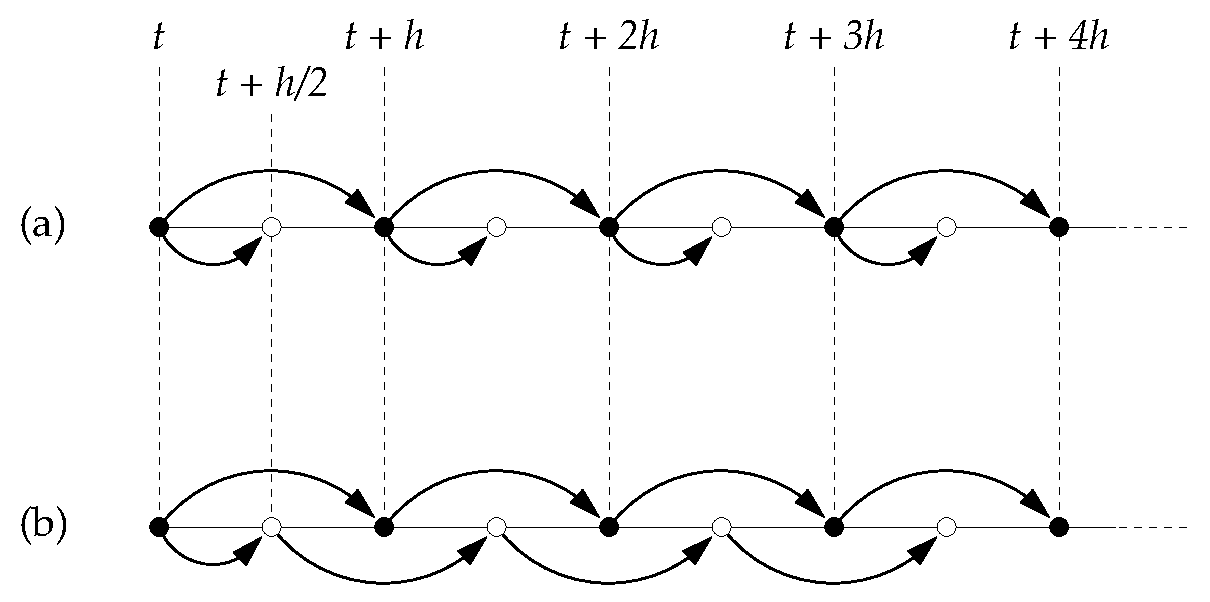
\includegraphics[width=0.8\textwidth]{./fig8-9.eps}}  
\centerline{\includegraphics[width=0.8\textwidth]{./leapfrog.pdf}}
\end{frame}

\begin{frame}{Leapfrog Method}

  \begin{itemize}
    \item The leapfrog method is a second-order algorithm.
  \item  Given the initial conditions $x(0)=x_0$ and $v(0)=v_0$, we can update the position and velocity at each time step $\Delta_t$:
  \begin{align*}
    & v_{n+1 / 2}=v_n+\frac{1}{2} \Delta_t a_n, \\
    & x_{n+1}=x_n+\Delta_t v_{n+1 / 2} \\
    & v_{n+1}=v_{n+1 / 2}+\frac{1}{2} \Delta_t a_{n+1},
    \end{align*}
    
    where $x_n=x(n\Delta_t)$, $v_n=v(n\Delta_t)$, and $a_n=a(n\Delta_t)=F(x_n,v_n,n\Delta_t)/m$.
  
    \item We need to use Euler's method to obtain $v_{-1/2}$.
\end{itemize}

%\centerline{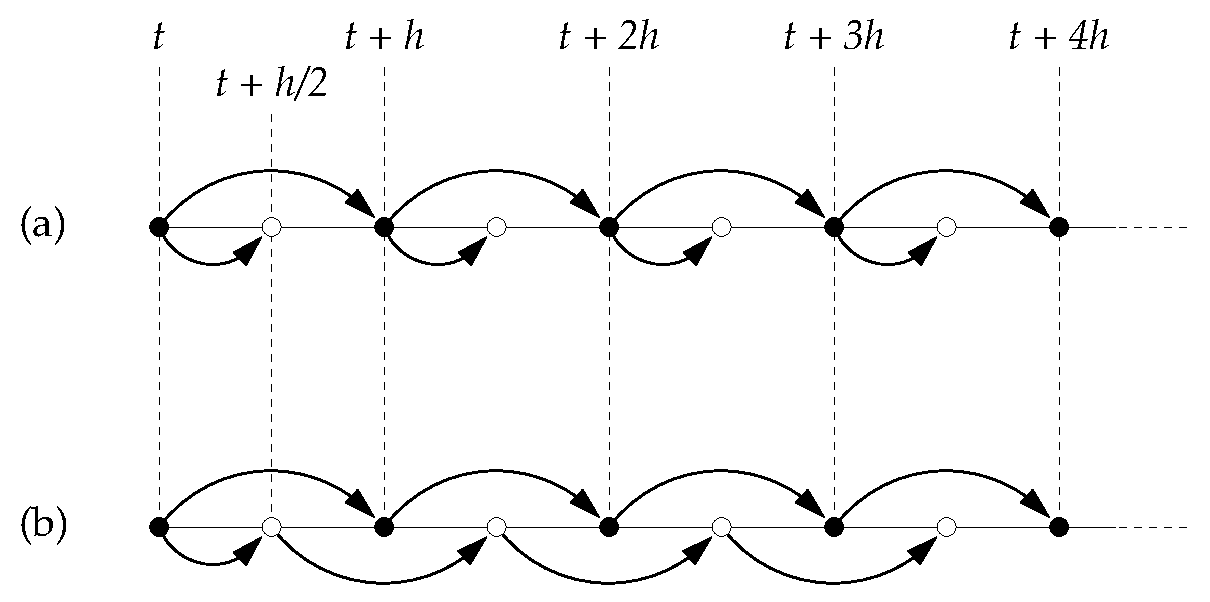
\includegraphics[width=0.8\textwidth]{./fig8-9.eps}}  
\end{frame}



\begin{frame}{Error Analysis}
  \begin{itemize}
    \item Forward and backward $x$ steps 
    \beforeverb
    \begin{align*} 
      & x_{n+1}=x_n+\Delta_t v_n+\frac{\Delta_t^2}{2} a_n+\frac{1}{6} 
      \Delta_t^3 \dot{a}_n+O\left(\Delta_t^4\right) \\ 
     +) \quad & x_{n-1}=x_n-\Delta_t v_n+\frac{\Delta_t^2}{2} a_n-\frac{1}{6} 
      \Delta_t^3 \dot{a}_n+O\left(\Delta_t^4\right)  
    \end{align*}
    \afterverb
    $\Rightarrow\quad   x_{n+1}=2 x_n-x_{n-1}+\Delta_t^2 a_n+O\left(\Delta_t^4\right)$
    \item Consider
    \beforeverb
    \begin{align*}
     & x_n-x_{n-1}=x\left(t_{n-\frac{1}{2}}+\frac{\Delta_t}{2}\right)-x\left(t_{n-\frac{1}{2}}-\frac{\Delta_t}{2}\right) \\
      &= \left[x_{n-\frac{1}{2}}+\left(\frac{\Delta_t}{2}\right) v_{n-\frac{1}{2}}+\frac{1}{2}\left(\frac{\Delta_t}{2}\right)^2 a_{n-\frac{1}{2}}+\frac{1}{6}\left(\frac{\Delta_t}{2}\right)^3 \dot{a}_{n-\frac{1}{2}}+\ldots\right]  \\
      & \quad-\left[x_{n-\frac{1}{2}}-\left(\frac{\Delta_t}{2}\right) v_{n-\frac{1}{2}}+\frac{1}{2}\left(\frac{\Delta_t}{2}\right)^2 a_{n-\frac{1}{2}}-\frac{1}{6}\left(\frac{\Delta_t}{2}\right)^3 \dot{a}_{n-\frac{1}{2}}+\ldots\right] \\
      &= \Delta_t v_{n-\frac{1}{2}}+O\left(\Delta_t^3\right) 
      \end{align*}
   \afterverb
   
   $ \Rightarrow \quad x_n-x_{n-1}=v_{n-\frac{1}{2}} \Delta_t+O\left(\Delta_t^3\right)$ 
    \end{itemize}
\end{frame}
\begin{frame}
  \begin{itemize}
    \item We have 
    \begin{align*}
      & x_{n+1}=2 x_n-x_{n-1}+\Delta_t^2 a_n+O\left(\Delta_t^4\right) \\
      & x_n-x_{n-1}=v_{n-\frac{1}{2}} \Delta_t+O\left(\Delta_t^3\right) \\
      & x_{n+1}=x_n+\Delta_t\left(v_{n-\frac{1}{2}}+\Delta_t a_n\right)\\
      \Rightarrow \quad & 
          v_{n-\frac{1}{2}}=\frac{1}{\Delta_t}\left(x_n-x_{n-1}\right)+O\left(\Delta_t^2\right) \\
          & x_{n+1}=x_n+\Delta_t\left(v_{n-\frac{1}{2}}+\Delta_t a_n\right)
    \end{align*}
    \item The error in each step $x_{n+1}$ is  $O(\Delta_t^3)$. 
  \end{itemize}
\end{frame}
\begin{frame}{Verlet Algorithm}
  \begin{itemize}
    \item The form without explicit $v$ is called the Verlet algorithm.
    \[
    x_{n+1}=2 x_n-x_{n-1}+\Delta_t^2 a_n+O\left(\Delta_t^4\right),
    \]
    with initial conditions $x_0$ and $x_1$.
    \item Velocity can be obtained by 
    \[ 
    v_{n+\frac{1}{2}}=\frac{x_{n+1}-x_{n-1}}{2\Delta_t}+O\left(\Delta_t^2\right).
    \]
    \item This algorithm is not often used because it is more susceptible to roundoff errors.
\end{itemize}
\end{frame}
\begin{frame}{Accumulated Error}
  \begin{itemize}
    \item The number of time steps is $N=T/\Delta_t$.
    \item Write the position at time step $n$ as the exact value plus an error:$x_n=x_n^\mathrm{ex}+\epsilon_n$.
    \item In the Verlet algorithm,
    \begin{align*}
      & x_{n+1}=2 x_n-x_{n-1}+\Delta_t^2 a_n+O\left(\Delta_t^4\right) \rightarrow \\
      & x_{n+1}^{\mathrm{ex}}-2 x_n^{\mathrm{ex}}+x_{n-1}^{\mathrm{ex}}=-\left(\delta_{n+1}-2 \delta_n+\delta_{n-1}\right)+\Delta_t^2 a_n+O\left(\Delta_t^4\right).
    \end{align*}
    \item  Replacing the discrete time derivatives by continuous ones, we have
    $$
    \ddot{x}^{\mathrm{ex}}(t)=-\ddot{\delta}(t)+a(t)+O\left(\Delta_t^2\right),
    $$
    and 
    $$ 
    \ddot{\delta}(t)=O\left(\Delta_t^2\right).
    $$
    The overall error in Verlet/Leapfrog algorithm is $O(\Delta_t^2)$.
  \end{itemize}
 \end{frame}
 


 \begin{frame}{Hamiltonian Flow is Symplectic}
  \begin{itemize}
    \item The Hamiltonian equations of motion are
    \begin{align*}
      \dot{x} &=\frac{\partial H}{\partial p}, \\
      \dot{p} &=\frac{\partial H}{\partial x}.
    \end{align*}
    \item From Liouville's theorem, the volume of phase space is conserved; that is the determinant of the Jacobian of the transformation from $(x,p)$ to $(x',p')$ is 1.
  \end{itemize}
  \centerline{\includegraphics[width=0.6\textwidth]{./symplectic.pdf}}

 \end{frame}
 \begin{frame}{Sympletic Integrator}
  \begin{itemize}
  \item Consider applying the leapfrog method to two close-by points in phase space $(x_0,v_0)$ and $(x_0+\delta x_0,v_0+\delta v_0)$.
    \[
    v_{1 / 2}+\delta v_{1 / 2}=v_0+\delta v_0+\frac{h}{2} F\left(x_0+\delta x_0\right), \quad v_{1 / 2}=v_0+\frac{h}{2} F\left(x_0\right),
    \]
    we have
    $$
\binom{\delta x_0}{\delta v_{1 / 2}}=A\binom{\delta x_0}{\delta v_0}, \quad
A=\left(\begin{array}{cc}
1 & 0 \\
\frac{h}{2} F^{\prime}\left(x_0\right) & 1
\end{array}\right) .
$$
\item Also, 
$$
\binom{\delta x_1}{\delta v_{1 / 2}}=B\binom{\delta x_0}{\delta v_{1 / 2}}, \quad B=\left(\begin{array}{ll}
  1 & h \\
  0 & 1
  \end{array}\right),
$$
and 
$$
\binom{\delta x_1}{\delta v_1}=C\binom{\delta x_1}{\delta v_{1 / 2}}, \quad C=\left(\begin{array}{cc}
  1 & 0 \\
  \frac{h}{2} F^{\prime}\left(x_1\right) & 1
  \end{array}\right)
$$

  \end{itemize}
 \end{frame}


 \begin{frame}{Sympletic Integrator}
  \begin{itemize}
  \item The final transformation is 
  \[
  \binom{\delta x_1}{\delta v_1}=J\binom{\delta x_0}{\delta v_0},
  \]
  where $J=ABC$ is the Jacobian of the transformation from $(x_0, v_0)$ to $(x_1, v_1)$.
  \item The determinant of $J$ is 1, which means that the leapfrog method conserves the volume of phase space.

  \end{itemize}
 \end{frame}
 \begin{frame}{Comparison with other integrators}
  \begin{itemize}
\item The advantage of symplectic algorithms is that they possess global stability. Since the area
bounded by adjacent trajectories is preserved, the trajectories do not diverge.
\item Non-symplectic algorithms, such as the Euler method, do not conserve the volume of phase space, and the trajectories can diverge.
\item Even RK2 and RK4, which are non-symplectic, the energy will drift over time.
  \end{itemize}
 
 \end{frame}
 \begin{frame}{Time Reversal Symmetry} 
 
  \begin{itemize}
    \item The algorithm is reversible in time, which means that we can run the simulation backwards.
    \begin{align*}
      & v_{n+1 / 2}=v_n+\frac{1}{2} \Delta_t a_n, \\
      & x_{n+1}=x_n+\Delta_t v_{n+1 / 2} \\
      & v_{n+1}=v_{n+1 / 2}+\frac{1}{2} \Delta_t a_{n+1}.
      \end{align*}
  \end{itemize}
  \centerline{\includegraphics[width=0.6\textwidth]{./TimeReversal.pdf}}
 \end{frame}

 \begin{frame}{Motions in two or three dimensions}
  \begin{itemize}
    \item The leapfrog method can be generalized to two or three dimensions.
    \item The position and velocity are now vectors: $\mathbf{x}(t)$ and $\mathbf{v}(t)$.
    \item The leapfrog algorithm is
    \item Given the initial conditions $\mathbf{x}(0)=\mathbf{x}_0$ and $\mathbf{v}(0)=\mathbf{v}_0$, we can update the position and velocity at each time step $\Delta_t$:
    \begin{align*}
      & \mathbf{v}_{n+1 / 2}=\mathbf{v}_n+\frac{1}{2} \Delta_t \mathbf{a}_n, \\
      & \mathbf{x}_{n+1}=\mathbf{x}_n+\Delta_t \mathbf{v}_{n+1 / 2}, \\
      & \mathbf{v}_{n+1}=\mathbf{v}_{n+1 / 2}+\frac{1}{2} \Delta_t \mathbf{a}_{n+1}.
    \end{align*}
  \end{itemize}
 \end{frame}
 \begin{frame}{Example: Planetary motion}
\begin{itemize}
  \item The force on a planet is given by
  \[\mathbf{F}=-\frac{G M m}{r^2} \hat{\mathbf{r}},
  \]
  where $M$ is the mass of the sun, $m$ is the mass of the planet, and $r$ is the distance between the planet and the sun.
  \item Assume $M\gg m$, we have the equations of motion for the planet:
  \begin{align*}
    \dot{x} & =v_x, \\
    \dot{v}_x & =-G M x / r^3, \\
    \dot{y} & =v_y \\
    \dot{v}_y & =-G M y / r^3,
    \end{align*}
    where $r=\sqrt{x^2+y^2}$.
  
\end{itemize}
  
 \end{frame}
 \begin{frame}{Example:Planetary motion}
  \begin{itemize}
    \item  The leapfrog algorithm gives
    \begin{align*}
      v_x(n+1 / 2) & =v_x(n-1 / 2)-\Delta_t G M x(n)\left[x^2(n)+y^2(n)\right]^{-3 / 2}, \\
      x(n+1) & =x(n)+\Delta_t v_x(n+1 / 2), \\
      v_y(n+1 / 2) & =v_y(n-1 / 2)-\Delta_t G M y(n)\left[x^2(n)+y^2(n)\right]^{-3 / 2}, \\
      y(n+1) & =y(n)+\Delta_t v_y(n+1 / 2) .
      \end{align*}
  \end{itemize}
 \end{frame}
 \begin{frame}{Hybid Monte Carlo}
  \begin{itemize}
    \item In the simulations of lattice gauge theories,  one of the most popular algorithms is the hybrid Monte Carlo or Hamiltonian Monte Carlo (HMC) algorithm.
    \item The leapfrog algorithm is used to generate new gauge field configurations.
  \end{itemize}
 \end{frame}
 \begin{frame}{Overview of Lattice Gauge Theory}
  \begin{itemize}
      \item \textbf{Lattice Discretization}:
      \begin{itemize}
          \item Space-time is represented as a finite grid (lattice) of points.
          \item Fields (e.g., gauge fields) are associated with the links between lattice points.
      \end{itemize}
      \item \textbf{Action \(S[U]\)}:
      \begin{itemize}
          \item Defines the energy of a field configuration.
          \item Example: Wilson action for gauge fields.
      \end{itemize}
      \item \textbf{Path Integral Approach}:
      \[
      Z = \int \mathcal{D}U \, e^{-S[U]}.
      \]
      \item \textbf{Goal}: Evaluate this path integral by sampling field configurations from the probability distribution:
      \[
      P(U) \propto e^{-S[U]}.
      \]
  \end{itemize}
\end{frame}

% Slide 2: Role of HMC
\begin{frame}{Role of HMC}
  \begin{itemize}
      \item Lattice gauge theory involves high-dimensional spaces of gauge field configurations.
      \item Traditional MCMC methods (e.g., Metropolis-Hastings) are inefficient due to random-walk behavior.
      \item HMC overcomes this inefficiency by:
      \begin{itemize}
          \item Leveraging gradients of the action \(S[U]\) to make informed moves.
          \item Simulating trajectories in the configuration space, avoiding local traps.
      \end{itemize}
      \item By using Hamiltonian dynamics, HMC efficiently explores the target distribution.
  \end{itemize}
\end{frame}

% Slide 3: HMC Framework in Lattice Gauge Theory
\begin{frame}{HMC Framework in Lattice Gauge Theory}
  \begin{enumerate}
      \item \textbf{Augment with Momentum Variables}:
      \begin{itemize}
          \item Introduce auxiliary momentum variables \(P\) for each gauge field configuration \(U\).
          \item Define the Hamiltonian:
          \[
          H(U, P) = S[U] + \frac{1}{2} P^T M^{-1} P,
          \]
          where \(M\) is a mass matrix (often identity).
      \end{itemize}
      \item \textbf{Hamilton's Equations}:
      \[
      \frac{dU}{dt} = \frac{\partial H}{\partial P}, \quad \frac{dP}{dt} = -\frac{\partial H}{\partial U}.
      \]
      \item \textbf{Leapfrog Integration}:
      \begin{itemize}
          \item Numerically solve Hamilton's equations using a symplectic integrator.
          \item Ensures reversibility and volume preservation.
      \end{itemize}
  \end{enumerate}
\end{frame}

% Slide 4: Sampling Process in HMC
\begin{frame}{Sampling Process in HMC}
  \begin{enumerate}
      \item \textbf{Initialize}:
      \begin{itemize}
          \item Start with a gauge field configuration \(U\).
          \item Sample momentum \(P\) from a Gaussian distribution.
      \end{itemize}
      \item \textbf{Simulate Trajectories}:
      \begin{itemize}
          \item Use the leapfrog algorithm to simulate the motion in \(U\)-\(P\) space.
          \item Compute gradients of the action \(S[U]\) for updates.
      \end{itemize}
      \item \textbf{Metropolis Acceptance Step}:
      \begin{itemize}
          \item Compute change in Hamiltonian:
          \[
          \Delta H = H(U', P') - H(U, P).
          \]
          \item Accept the new configuration with probability:
          \[
          \min(1, e^{-\Delta H}).
          \]
      \end{itemize}
      \item \textbf{Iterate}:
      \begin{itemize}
          \item Generate a sequence of accepted configurations to approximate the target distribution.
      \end{itemize}
  \end{enumerate}
\end{frame}
\begin{frame}{Sampling}
    \centering
    \animategraphics[loop,width=0.8\textwidth]{10}{animation/HMC}{1}{226}
\end{frame}
% Slide 5: Why HMC is Suitable for Lattice Gauge Theory
\begin{frame}{Why HMC is Suitable for Lattice Gauge Theory}
  \begin{itemize}
      \item \textbf{High-Dimensional Spaces}:
      \begin{itemize}
          \item Gauge field configurations involve thousands of degrees of freedom.
          \item HMC scales well with dimensionality.
      \end{itemize}
      \item \textbf{Gradient-Based Efficiency}:
      \begin{itemize}
          \item Uses \(\nabla S[U]\) to guide exploration of the configuration space.
          \item Avoids inefficient random walks.
      \end{itemize}
      \item \textbf{Preservation of Gauge Symmetry}:
      \begin{itemize}
          \item HMC respects the symmetry structure of lattice gauge theories.
      \end{itemize}
      \item \textbf{Large Acceptance Rates}:
      \begin{itemize}
          \item Well-tuned step sizes and trajectory lengths result in high acceptance rates.
      \end{itemize}
  \end{itemize}
\end{frame}


% Slide 7: Challenges and Advances
\begin{frame}{Challenges and Advances}
  \begin{itemize}
      \item \textbf{Parameter Tuning}:
      \begin{itemize}
          \item Step size and trajectory length must balance efficiency and accuracy.
      \end{itemize}
      \item \textbf{Critical Slowing Down}:
      \begin{itemize}
          \item Near phase transitions, convergence slows down.
          \item Mitigation: Multigrid methods, adaptive step sizes.
      \end{itemize}
      \item \textbf{Preconditioning}:
      \begin{itemize}
          \item Improved mass matrix designs enhance performance in high dimensions.
      \end{itemize}
      \item \textbf{Computational Cost}:
      \begin{itemize}
          \item Lattice gauge theory requires significant computational resources.
          \item Mitigation: Parallel computing and specialized algorithms.
      \end{itemize}
  \end{itemize}
\end{frame}

\end{document}


